\documentclass[a4paper, 12pt, garamond]{book}
\usepackage{cours-preambule}

\dominitoc
\faketableofcontents

\makeatletter
\renewcommand{\@chapapp}{Fiches -- numéro}
\makeatother

\begin{document}
\setcounter{chapter}{5}

\chapter{Python et incertitudes par simulation \textsc{Monte-Carlo}}

\vfill

\begin{prgm}
  \begin{tcb}*(ror)"how"{Savoir-faire}
    \begin{itemize}[label=$\diamond$, leftmargin=10pt]
      \item Simuler, à l’aide d’un langage de programmation ou d’un tableur, un
        processus aléatoire permettant de caractériser la variabilité de la
        valeur d’une grandeur composée.
      \item Simuler, à l’aide d’un langage de programmation ou d’un tableur, un
        processus aléatoire de variation des valeurs expérimentales de l’une des
        grandeurs – simulation \textsc{Monte-Carlo} – pour évaluer l’incertitude
        sur les paramètres du modèle.
    \end{itemize}
  \end{tcb}
\end{prgm}

\vfill
\minitoc
\vfill

\newpage

\section{Survivre en \texttt{Python}}
\subsection{Les bases}
\subsubsection{Calcul et affichage basiques}
\begin{python}
# Ce qui est après un # est un commentaire, et non traité dans le code

a = 2       # affecte la valeur 2 à la variable globale a
b = 3*a     # b vaut 3*2 = 6. Si on change la valeur de a, on devra recalculer b
c = a**3    # ** indique une puissance, ici puissance 3 (donc c = 8)
d = 5.5e-3  # eNBRE est un raccourci pour 10^(NBRE). Ici, d = 0.0055.
\end{python}

\subsubsection{Fonctions basiques}
\begin{python}
print(d)               # affiche la valeur de d
print(f'd = {d}')      # affiche "d = 0.0055"
print(f'd = {d:.2f}')  # affiche "d = 0.01" : décimal 2 chiffres après ','
print(f'd = {d:.2e}')  # affiche "d = 5.50e-03" : scientifique 2 décimales

type(a)   # donne le type d'objet de la variable a : int (entier)
type(d)   # donne le type d'objet de la variable d : float (décimal)

abs(-3)         # donne la valeur absolue d'un nombre : 3

len([1, 2, 3])  # donne la longueur d'une liste : 3
min([1, 2, 3])  # donne la valeur minimale d'une liste : 1
max([1, 2, 3])  # donne la valeur maximale d'une liste : 3
\end{python}

\subsection{Gestion de données}
\subsubsection{Listes}

\begin{python}
L = [1, 2, 3]  # créé la liste L contenant les valeurs 1, 2 et 3
print(L[0])    # extrait la première valeur de L : 1
print(L[-1])   # extrait la dernière valeur de L : 3
print(L[:2])   # extrait les deux premières valeurs de L : 1 et 2
print(L[1:])   # extrait toutes les valeurs à partir de la deuxième : 2 et 3

L.append(42)    # ajoute l'élément 42 à la fin de la liste
L2 = L + [5, 6] # concatène la liste L et la liste [5, 6] dans une nouvelle
print(L2)       # [1, 2, 3, 42, 5, 6]
\end{python}

\subsubsection{Tableaux et \texttt{numpy}}
\begin{python}
import numpy as np

tab = np.array([1, 2, 3])  # créé le tableau [1, 2, 3]
tab+1                      # ajoute 1 à toutes les valeurs de tab
tab*2e-3                   # multiplie toutes les valeurs de tab par 0.002
np.sqrt(tab)               # applique racine carré à tous les éléments de tab
np.exp(tab)                # exponentielle
np.log(tab)                # logarithme NÉPÉRIEN (ln français)
np.log10(tab)              # logarithme décimal (log français)

np.linspace(min, max, nbre) # découpe [min, max] en nbre parties égales
np.mean(tab)                # donne la valeur moyenne de tab
np.std(tab, ddof=1)         # donne l'écart-type de tab

np.polyfit(X, Y, 1)         # donne les coefficients a et b de Y = a*X+b
\end{python}

\subsection{Automatisation}
\subsubsection{Fonctions personnelles}
\begin{python}
def puissance(arg1, arg2): # définit la fonction puissance de 2 arguments
    resultat = arg1**arg2  # variable locale de calcul
    return(resultat)       # fin de la fonction, résultat final

print(puissance(2, 3))     # donne le résultat du calcul : 8

def comparaison(x,y):
    if x > y:                                    # condition d'exécution
        print("argument 1 supérieur au second")  # si oui, exécute
    elif x < y:                                  # sinon, autre condition
        print("argument 1 inférieur au second")  # si oui, exécute
    else:                                        # pour tous les autres cas,
        print("argument 1 égal au second")       # exécute

print(comparaison(1,2))    # "argument 1 inférieur au second"
\end{python}

\subsubsection{Boucles \texttt{for}}
\begin{python}
for i in range(10):   # créé i qui commence à 0, terminera à 9, et augmente
                      # de 1 à chaque réalisation des lignes en-dessous
    print(i)          # affichera 0, puis 1, puis 2, et jusqu'à 9

L = []                # liste vide
for i in range(3):    # exécute la suite 3 fois : i=0, puis 1, puis 2
    L.append(3*i)     # ajoute 3*i à la fin de la liste
print(L)              # [0, 3, 6]

for i, k in enumerate(L):  # i compte à partir de 0, k prend les valeurs de L
    print(f'L[{i}] = {k}') # L[0] = 0, L[1] = 3, L[2] = 6

L2 = [3*i for i in range(3)] # créé L d'une manière plus compacte
print(L2)                    # même résultat
\end{python}

\subsection{Tracé de graphiques}
\subsubsection{Minimal}
\begin{python}
import matplotlib.pyplot as plt

abscisse = np.linspace(0, 10, 8) # définit les abscisses qu'on tracera
ordonnee = abscisse**2           # et les ordonnées

plt.plot(abscisse, ordonnee)     # place les points, les relie par des segments
plt.xlabel('t (s)')              # nomme l'abscisse
plt.ylabel('x (m)')              # nomme l'ordonnée

plt.show()                       # obligé pour afficher
\end{python}

\begin{minipage}[t]{.48\linewidth}
  ~
  \begin{center}
    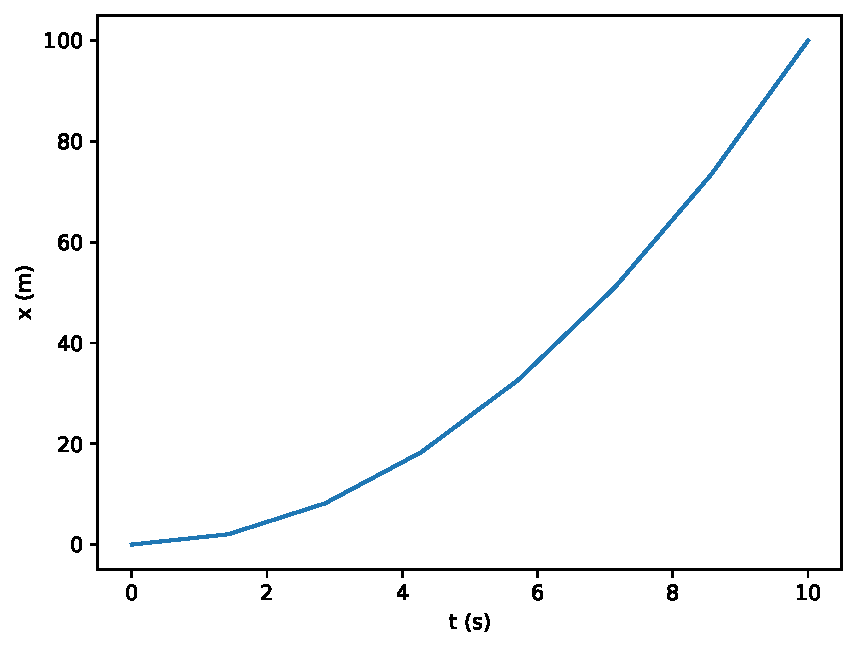
\includegraphics[width=\linewidth]{figures/python_plt-1}
    \captionof{figure}{Figure minimale.}
    \label{fig:mini}
  \end{center}
\end{minipage}
\hfill
\begin{minipage}[t]{.48\linewidth}
  ~
  \begin{center}
    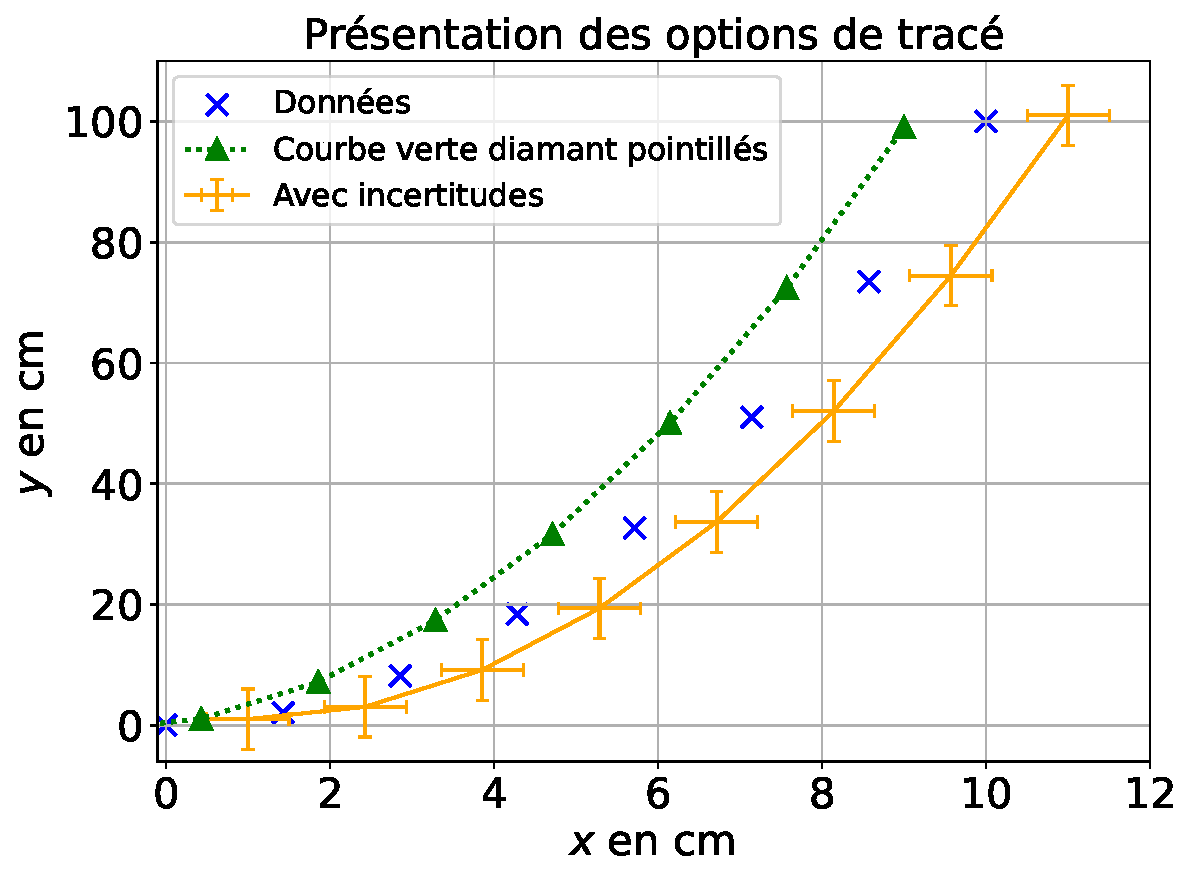
\includegraphics[width=\linewidth]{figures/python_plt-2}
    \captionof{figure}{Figure complexe.}
    \label{fig:cplx}
  \end{center}
\end{minipage}

\subsubsection{Total}
\begin{python}
X = np.linspace(0, 10, 8)
Y = X**2

plt.figure(figsize=(8, 6))     # dimension horizontale, verticale
plt.grid()                     # affiche un quadrillage de lecture
plt.xticks(fontsize=20)        # affiche les nombres de l'axe x plus grand
plt.yticks(fontsize=20)        # affiche les nombres de l'axe y plus grand
plt.xlabel('$x$ en cm',        # Donne le nom de l'axe x, $ pour le mode math
           fontsize=20)        # en grand
plt.ylabel('$y$ en cm',        # Donne le nom de l'axe y, $ pour le mode math
           fontsize=20)        # en grand

plt.scatter(X, Y,              # nuage de points X en abscisse et Y en ordonnée
            marker='x', s=100, # possibilité de customiser le tracé
            color='blue',      # pour la couleur
            label='Données')   # pour la légende

plt.errorbar(X+1, Y+1,         # nuage de points X abscisse et Y ordonnée
             xerr=.5,          # incertitude en x
             yerr=5,           # incertitude en y
             capsize=3,        # indique la limite des erreurs
             color='orange',   # pour la couleur
             label='Avec incertitudes')

plt.plot(X-1, Y-1,             # graphique relié
         color="g",            # couleur
         marker="^",           # marker
         markersize=10,        # taille marker
         linestyle="dotted",   # type de ligne
         linewidth=2,          # épaisseur
         label="Courbe verte diamant pointillés")

plt.title('Présentation des options de tracé',
          fontsize=20)
plt.legend(fontsize=15)

plt.tight_layout()             # évite les débordements ou rognages
plt.xlim(min(X)-.1, max(X)+2)  # pour les limites d'affichage en abscisse
plt.ylim(min(Y)-6, max(Y)+10)  # pour les limites d'affichage en ordonnée
plt.show()
\end{python}

\section{Simulations \textsc{Monte-Carlo}}
\subsection{Principe}
On dispose généralement de plusieurs jeux de données pour
lesquels on a des incertitudes de mesure, et on veut calculer $z$ qui dépend de
ces données mais d'une manière complexe\ftn{Comprendre~: pas donnée dans la fiche
\texttt{Mesures et incertitudes}}. On peut alors réaliser une simulation.

En effet, connaissant l'intervalle d'existence des mesures, on peut prendre
aléatoirement d'autres valeurs possibles pour les mesures, et faire toute une
série de calculs avec des valeurs légèrement modifiées. On pourra alors
finalement prendre la moyenne des valeurs calculées et leur écart-type pour
avoir la propagation des incertitudes~!

\begin{tcb}(ror){Cœur de la simulation}
  Finalement, le cœur de la simulation revient (presque) à réaliser une estimation
  d'incertitude de type A sur les valeurs calculées~!
\end{tcb}

\subsection{Application~: mesure d'une distance focale}
On peut mesurer la focale d'une lentille convergente par la méthode de
\textsc{Bessel}~:
\[
  \boxed{f' = \frac{D^{2}-d^{2}}{4D}}
\]
avec $d$ la plage de positions de la lentille qui garde une image nette sur
l'écran, et $D$ la distance objet-écran. S'il est possible de faire le calcul
analytique ici, il peut être plus rapide de réaliser une propagation des
incertitudes des valeurs $d$ et $D$ sur la valeur calculée de $f'$.

Pour cela,
\begin{itemize}[label=$\diamond$, leftmargin=10pt]
  \item On note les valeurs extrêmes de $d$ dans une liste \texttt{D\_d}~;
  \item On note les valeurs extrêmes de $D$ dans une liste \texttt{D\_D}~;
  \item On créé une liste \texttt{liste\_f} vide qui accueillera les valeurs de
    $f'$ calculées~;
  \item On fixe $N \gtrsim \num{e4}$ le nombre de simulations~;
  \item Pour $i$ allant de 0 à $N-1$~:
    \begin{itemize}[label=$\triangleright$, leftmargin=10pt]
      \item On tire aléatoirement une valeur de $d$ dans l'intervalle
        \texttt{D\_d}~;
      \item On tire aléatoirement une valeur de $D$ dans l'intervalle
        \texttt{D\_D}~;
      \item On calcule $f'$ avec ces données \textbf{simulées}~;
      \item On ajoute cette valeur simulée à la liste des valeurs de $f'$.
    \end{itemize}
  \item On calcule alors la valeur moyenne des $f'$, qui sera la valeur la plus
    probable, et l'écart-type de la liste des $f'$, qui sera son
    incertitude-type.
\end{itemize}

La fonction \texttt{Python} qui permet de tirer aléatoirement une valeur entre
\texttt{min} et \texttt{max} est \texttt{np.random.uniform(min, max)}. Ainsi, en
\texttt{Python}~:
\begin{python}
d = 12               # cm
Delta_d = 0.1        # cm
D_d = [11.9, 12.1]   # cm
D = 50               # cm
Delta_D = 0.5        # cm
D_D = [49.5, 50.5]   # cm

N = 100000
liste_f = []
for i in range(0, N):
    d_simu = np.random.uniform(D_d[0], D_d[1])
    D_simu = np.random.uniform(D_D[0], D_D[1])
    f_simu = D_simu/4 - d_simu**2/(4*D_simu)
    liste_f.append(f_simu)

fmoy = np.mean(liste_f)
uf = np.std(liste_f, ddof=1)
print(f'f = {fmoy:.2f} +- {uf:.2f}')
\end{python}

\subsection{Application~: régression linéaire}
Prenons l'exemple de la régression linéaire~:
\[
  y = ax+b
\]
On a mesuré $x$ et $y$, et on obtient $a$ et $b$ avec \texttt{np.polyfit(x, y,
1)}. Mais ce calcul ne donne pas l'incertitude sur $a$ et $b$. Les deux valeurs
étant interdépendantes, on n'a pas d'expression analytique pour les
déterminer~: on va donc les simuler.

Chaque valeur de $x$ est comprise dans un certain intervalle $x \pm \Delta_x$,
et de même pour $y$. Plutôt que de prendre la valeur centrale et de calculer $a$
et $b$ avec ces valeurs, on peut essayer de calculer $a$ et $b$ pour des valeurs
de $x$ et de $y$ légèrement modifiées. On va donc réaliser un grand nombre de
régressions linéaires en modifiant les valeurs de $x$ et $y$, et on prendra la
moyenne des $a$ et $b$ comme étant la valeur centrale et leur écart-type pour
leur incertitude.

\subsection{En pratique}
\begin{itemize}[label=$\diamond$, leftmargin=10pt]
  \item On détermine les demi-largeurs $\Delta_x$ et $\Delta_y$. Si ce sont des
    incertitudes-types, on aura $\Delta_x = u(x)\sqrt{3}$. Sinon, c'est la plage
    de mesures valables.
  \item On fixe un nombre $N$ très grand.
  \item On créé des listes vides \texttt{liste\_a} et \texttt{liste\_b} pour y
    stocker les futures valeurs des $a$ et des $b$ calculés.
  \item Pour chaque $i$ compris entre $0$ et $N-1$~:
    \begin{itemize}[label=$\triangleright$]
      \item on prend \texttt{x\_simu} dans l'intervalle $[x-\Delta_x,
        x+\Delta_x]$~;
      \item on prend \texttt{y\_simu} dans l'intervalle $[y-\Delta_y,
        y+\Delta_y]$~;
      \item on calcule \texttt{a\_simu} et \texttt{b\_simu} avec ces valeurs
        simulées~;
      \item on les stocke dans \texttt{liste\_a} et \texttt{liste\_b}.
    \end{itemize}
  \item On a alors $N$ valeurs de $a$ et de $b$~: les valeurs les plus probables
    sont les moyennes, et leurs incertitudes-types sont les les écarts-types des
    listes de $a$ et de $b$.
\end{itemize}

Ainsi, en \texttt{Python}~:
\begin{python}
x = np.array([0,1,2,3,4, 5,6,7,8,9,10])
ux = 0.1*np.ones(len(x))   # incertitude de 0.1 sur chaque valeur

y = np.array([2.20,2.00,1.60,1.55,1.16, 1.00,0.95,0.60,0.36,0.36,0.18])
uy = 0.12*np.ones(len(y))  # incertitude de 0.12 sur chaque valeur

Delta_x = ux*np.sqrt(3)    # demi-largeur x
Delta_y = uy*np.sqrt(3)    # demi-largeur y

N = 10000                  # nombre de régressions à effectuer

liste_a, liste_b = [], []  # création des listes vides pour stocker les valeurs
for i in range(N):
    x_simu = x + np.random.uniform(-Delta_x, Delta_x)
    y_simu = y + np.random.uniform(-Delta_y, Delta_y)

    a_simu, b_simu = np.polyfit(x_simu, y_simu, 1)

    liste_a.append(a_simu)
    liste_b.append(b_simu)

a_moy, b_moy = np.mean(liste_a), np.mean(liste_b)
ua, ub = np.std(liste_a, ddof=1), np.std(liste_b, ddof=1)

print(f'Coef.directeur = {a_moy:.3e} +- {ua:.3e}')
print(f'Ordonnée à l'origine = {b_moy:.3e} +- {ub:.3e}')
\end{python}

\end{document}
